% \section{Serialization}

% \begin{figure}[t]
%   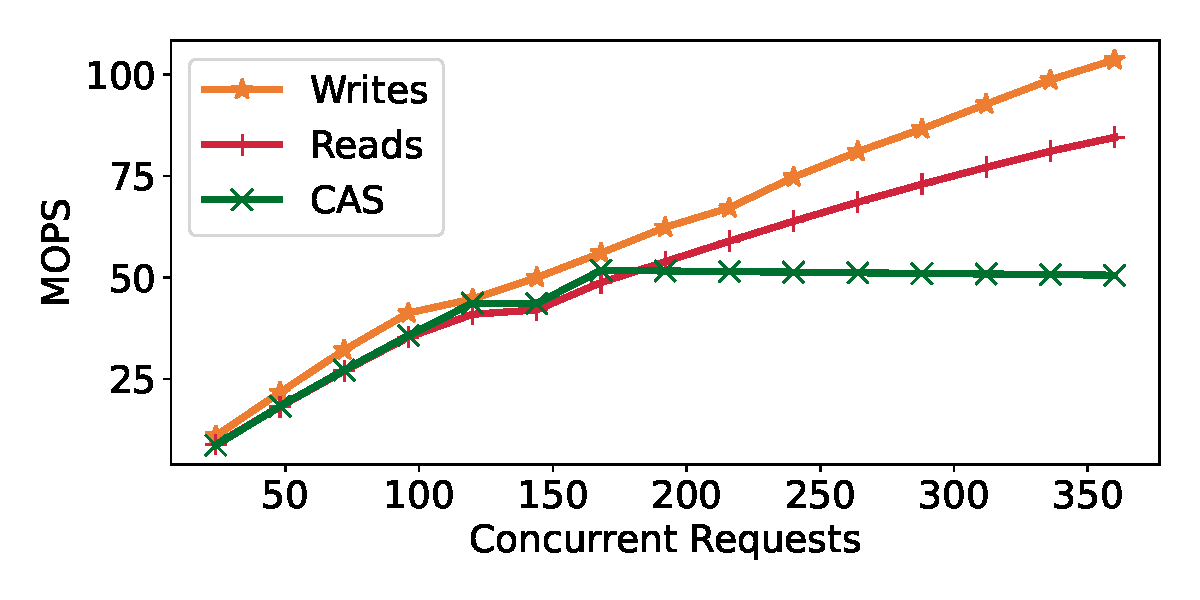
\includegraphics[width=0.485\textwidth]{fig/rdma_concur.pdf}
%   \vskip -0.5em

%     \caption{Achieved throughput of RDMA verbs across twenty queue
%       pairs on data-independent addresses as a function of request
%       concurrency.  When using atomic requests, ConnectX-5 NICs can
%       support approximately 2.7 MOPS per queue pair, up to about 55
%       MOPS in aggregate.}

%     \label{fig:rdma_concur}
%       \vskip -0.5em
% \end{figure}

% \begin{figure}[t]
%     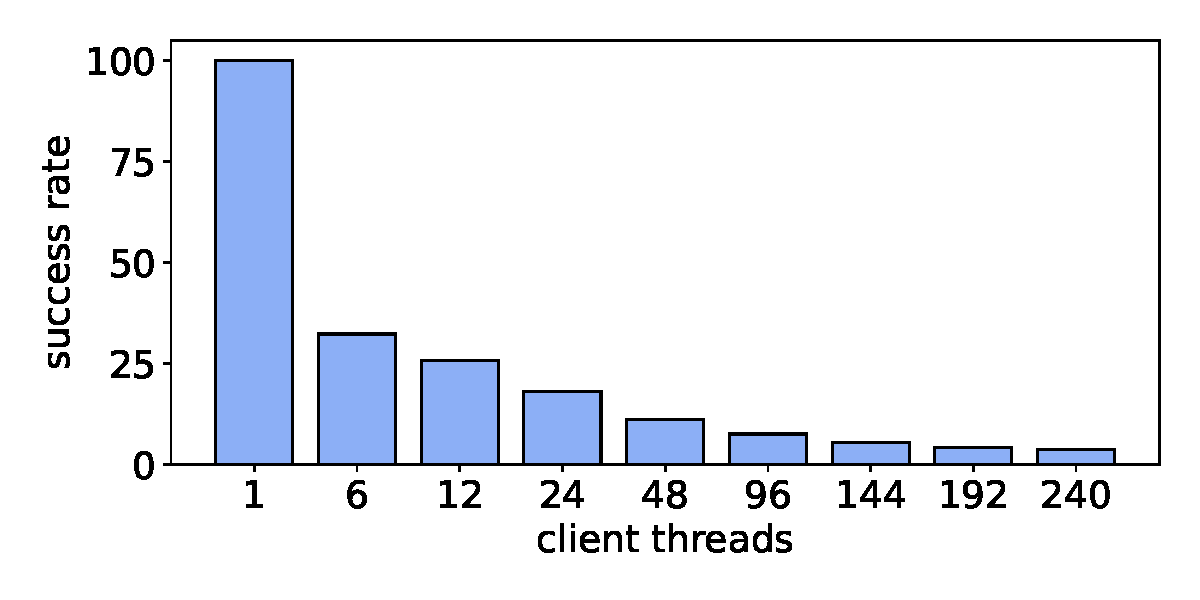
\includegraphics[width=0.485\textwidth]{fig/success_rate.pdf}
%     \vskip -0.5em
%     \caption{Percentage of successful operations in a
%       50:50 read-write workload spread across 1,024 keys according
%       to a Zipf(0.99) distribution as more client threads are
%       added. At 240 threads less than 4\% of operations succeed.}
      
%     \vskip -0.5em
%     \label{fig:success_rate}
% \end{figure}

% \begin{figure}[t]
%   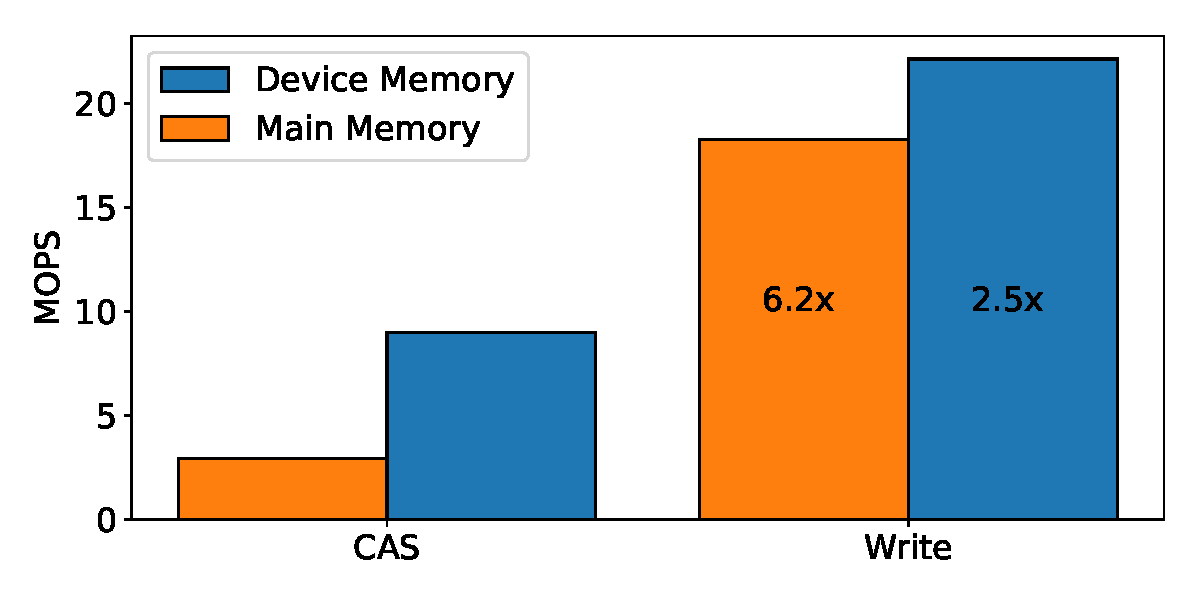
\includegraphics[width=0.485\textwidth]{fig/cas_vs_writes.pdf}
% %  \vskip -0.5em

%   \caption{ Throughput comparison of serialized RDMA operations in
%     NIC-mapped device and main memory. Writes obtain 6.2$\times$ higher
%     throughput than CAS in host memory and 2.5$\times$ higher in NIC memory despite being restricted to a single queue pair.  }

%     \label{fig:cas_vs_writes}
% %      \vskip -0.5em
% \end{figure}

% \subsection{RDMA serialization} 
% %%
% RDMA atomics instructions serialize remote memory operations
% without the need for a memory side CPU. These instructions
% \textit{Fetch-and-Add} and \textit{Compare-and-Swap} (CAS)
% execute on 64 bit width words and are guaranteed to have
% atomic visibility across all queue pairs. These operations
% are expensive. On a single address atomic instructions can
% only execute a few million operations per second, each
% operation forces a blocking PCIe round trip.  As a
% performance mitigation Mellanox NICs supply a small (few KB)
% region of device mapped memory which allows the memory side
% NIC to execute RDMA instructions on it's local device memory
% without incurring a PCIe round trip~\cite{sherman}.
% Executing atomics on this memory is 3x higher throughput
% than host memory, but still slower than it's read and write
% counterparts~\ref{fig:cas_vs_writes}.  Across independent
% addresses they have approximately half the throughput of
% read and write (Figure~\ref{fig:rdma_concur}).

% Data structures built on RDMA atomics have hard performance
% limits because the aforementioned constraints.  Locks
% located at a single address which use traditional lock,
% unlock operations are limited to around 500k accesses per
% second. This assumes perfectly coordinated requests, under
% contention requests which fail to acquire or release a lock
% still consume operation bandwidth.
% %%
% Under contention RDMA has poor support for traditional
% locking. In contrast optimistic data structures with locks
% scattered throughout, such as a linked list, are not rate
% limited by this single address restriction.  However, they
% are fundamentally limited by the fact that any atomics have
% half the throughput of reads and writes. More critically,
% under contention optimistic data structures have no liveness
% guarantees. We measure the failure rate of optimistic reads
% and writes to a shared linked list. Operations are reads and
% writes to the tail of the list, all writes are appends.
% under contention atomic operations fail frequently
% (Figure~\ref{fig:success_rate}).  RDMA has no support for
% resolving pointers (pointer chasing) and retrying operations
% for such data structures~\cite{rma,snap,prism}, a simple
% operation usually executed by a memory side CPU. As such
% RDMA clients are forced to resolve their failures requests
% themselves often retrying many times.
% %%
% Atomic operations are not the only serialization mechanism
% provided by RDMA. Reliable Connections provide in order
% delivery on individual queue pairs. This allows clients to
% issue multiple requests in parallel and allows the NIC to
% resolve reordering and dropped packets using go-back-n
% retransmission.  When clients are collocated, queue pairs
% can be shared by multiple cores through techniques such as
% flat combining~\cite{flock,sherman}. Flat combing removes
% the need for RDMA atomics, as clients can locally resolve
% their conflicts and then issue their requests as reads and
% writes.  Unfortunately this technique is not applicable to
% distributed clients as they do not share access to the same
% queue pair.


% \subsection{Overheads}

% \paragraph{Bandwidth inflation.} 
% %%
% One of the most direct impacts of failed requests is the
% bandwidth overhead of the retries. When atomic operations
% fail they must be retried.  In the case of locking the
% number of retries is a direct result of the critical section
% size, the number of clients, and the aforementioned
% operation limits. Each failed request consumes additional
% bandwidth. Bandwidth inflation in optimisitic schemes is
% proportial to the degree of contention. When optimistic
% operations fail they must be retried.
% %%
% Our measurements show that under contention the average
% bandwidth cost of Clover read and write operations can
% inflate by 16$\times$ (Figure~\ref{fig:bandwidth_reduction})
% when compared to an optimal scenario in which all operations
% succeed on their first try.

% % Because a Clover operation actually
% % consists of multiple RDMA requests, the total bandwidth is not
% % strictly proportional to the failure rate, but rather slightly
% % sub-linear.  Nevertheless, the expected cost of each operation rises
% % steadily with contention, which is a function of both the workload and
% % level of concurrency. 

% \paragraph{Tail latency.}

% Perhaps even more significant than the overheads associated with the expected
% number of retries is the cost at the tail---namely the latency associated with
% those particularly ``unlucky'' requests that fail repeatedly.  Note that these
% operations are precisely those for hot memory locations, so likely to be
% ones that matter.  Under contention
% %(e.g., 50\% write operations with 396 threads)
% Clover's 99th-percentile tail latency increases by
% over 300$\times$ (Figure~\ref{fig:tail_latency}) in our experiments.

% % \subsection{Programmable Switch Serialization}
% \section{In-network serialization}

% \begin{figure}[t]
%     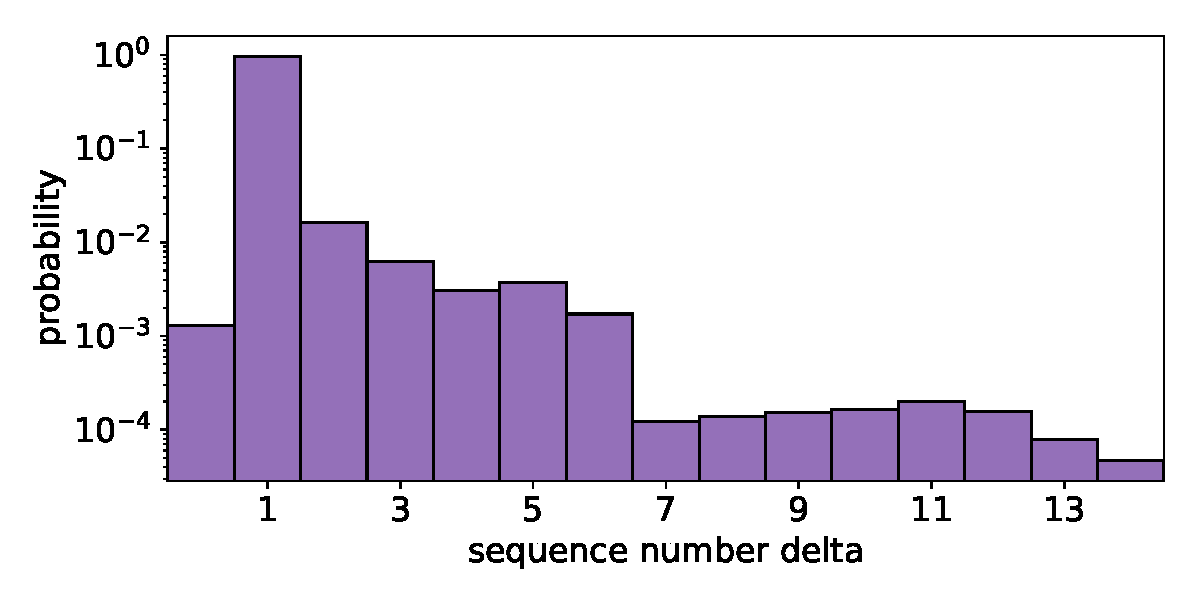
\includegraphics[width=0.485\textwidth]{fig/qp_reordering.pdf}
%   \vskip -0.5em    
%     \caption{PDF of request reorderings.  Retransmitted requests lead to reordering values of zero.   97\%
%     of requests retain their order (delta=1), however reorderings of up to 15
%     requests can occur. (Note logarithmic $y$ axis.)}
%   \vskip -0.5em
%     \label{fig:reorder}
% \end{figure}

% Switches can cheaply serialize packets~\cite{when-computer}.
% Programable switches with P4 pipelines can utilize this
% cheap serialization, along with their ability to manage
% small amounts of state in network, to serialize distributed
% applications. Mind for instance provides a unified TLB and
% cache for disaggregated applications~\cite{mind}. Packets
% processed by a programmable switch are sequenced in order,
% updates to the switches registers are atomic with respect to
% the packets as each state of the pipeline is occupied by
% exactly one packet at a time. A centralized switch can
% therefore apply monotonic sequence numbers to a stream of
% packets, maintain a lock, or keep a shared variable up to
% date without the need for explicit atomic operations.

% Unfortunately this serialization is not sufficient for RDMA
% memory operations out of the box. RDMA packets on two
% reliable connections may be ordered on the switch, and then
% subsequently reordered by the receiving side NIC, or by the
% PCIe bus~\cite{understanding-pcie}. NIC and PCIe reordering
% is not merely an academic concern!  Figure~\ref{fig:reorder}
% illustrates the extend of reordering across connections.
% This experiment uses an in network serializer to give each
% packet an incremental monotonic sequence number. The x axis
% measure the absolute delta between sequence number values on
% response packets.  The majority of packets remain ordered
% (sequence number 1), however significant reordering does
% occur up to 15 packets apart.

% Switches are not intended to be general purpose computers,
% their purpose is to forward packets. It is trivial to
% construct switch programs which consume it's few resources.
% Oversized caches step on the toes of packet buffers and lead
% to dropped packets, and complex logic requires packet
% recirculation which eats into the switches bandwidth.
% limiting it's ability to buffer, and process packets at full
% bandwidth.
% %%
% For example, terminating connections with a switch is
% prohibitively expensive as both the state of the entire
% connections, and the logic for connection startup and
% teardown would consume large quantities of the switches
% buffers. Any logic, or data offloaded to a programable
% switch must therefore be minimal in order to meet the
% compute and data restrictions of the switches SRAM.


\section{Serialization}

The fundamental challenge faced by passive remote memory systems is
ensuring consistency~\cite{ivy} by ordering accesses to any given
location.  RDMA reliable connections provide per-connection ordering,
enabling clients to
%Atomic operations are not the only serialization mechanism
%provided by RDMA. Reliable Connections provide in order
%delivery on individual queue pairs. This allows clients to
issue multiple outstanding requests; the NIC ensures in-order delivery despite 
packet reordering and drops with sequence numbers and go-back-$n$
retransmission.

\subsection{Per-connection throughput}

\begin{figure}[t]
  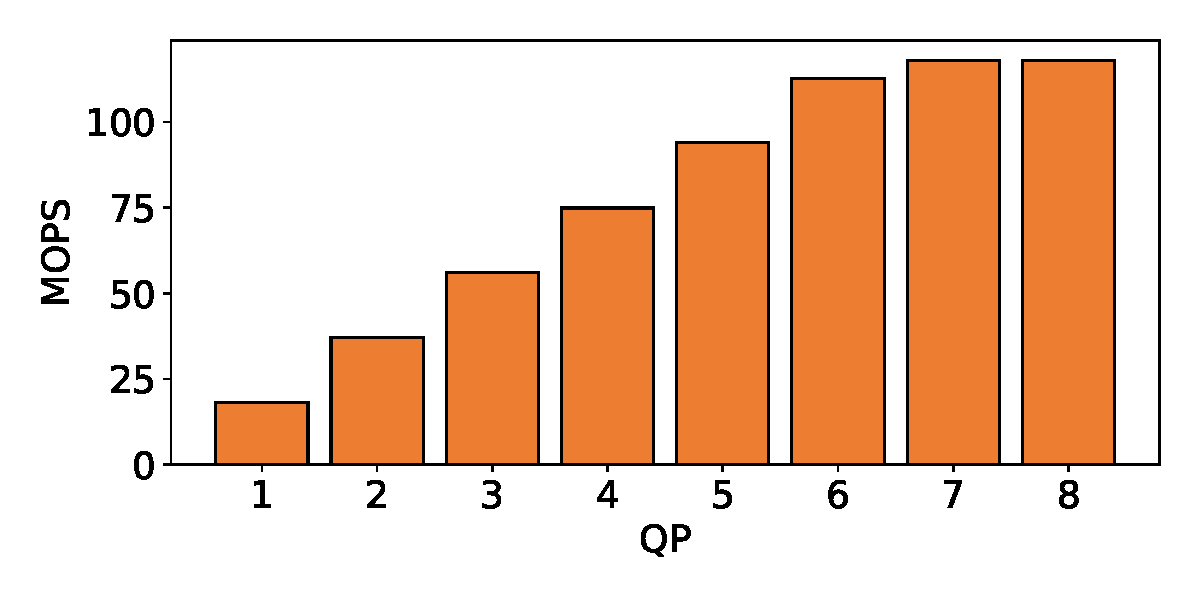
\includegraphics[width=0.485\textwidth]{fig/qp_bottleneck.pdf}
  \vskip -0.5em
\caption{Max throughput as a function of the number of RoCEv2 RC connections. Each QP gets a single
core, and issues in-lined writes. A single connection only offers a fraction of the
total NIC throughput.} 
  \vskip -0.5em
  \label{fig:qp_bottleneck}
\end{figure}

When clients are collocated, queue pairs
can be shared by multiple cores through techniques such as
flat combining~\cite{flock,sherman}.
%Flat combing removes
%the need for RDMA atomics, as clients can locally resolve
%their conflicts and then issue their requests as reads and
%writes.
Unfortunately Figure~\ref{fig:qp_bottleneck} shows that the
performance of individual queue pairs fall far short of line rate on
our NICs; we do not observe full performance until at least seven
queue pairs are used simultaneously. Moreover, as traditionally
conceived, a QP is intended to be established between a single client
and server---limiting its utility in a disaggregated setting.  In the
following subsections we experimentally illustrate the challenges to
ordering across such clients.


% \subsection{Programmable Switch Serialization}
\subsection{Switch-enforced ordering}

\begin{figure}[t]
    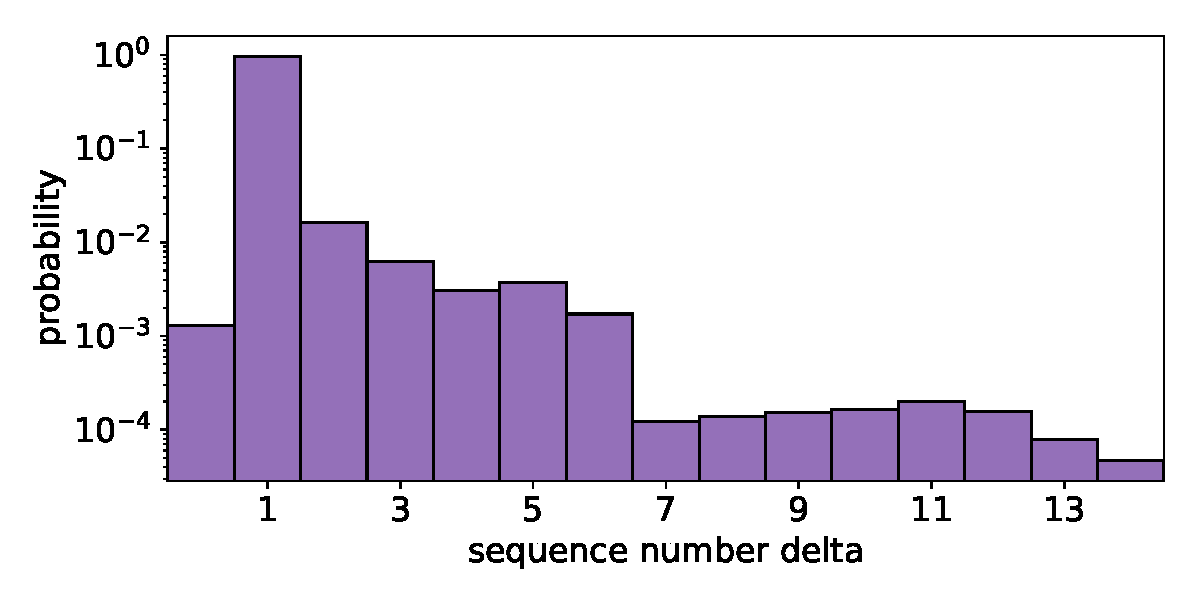
\includegraphics[width=0.485\textwidth]{fig/qp_reordering.pdf}
  \vskip -0.5em    
    \caption{PDF of request reorderings.  Retransmitted requests lead to reordering values of zero.   97\%
    of requests retain their order (delta=1), however reorderings of up to 15
    requests can occur. (Note logarithmic $y$ axis.)}
  \vskip -0.5em
    \label{fig:reorder}
\end{figure}

Packets processed by a programmable switch pipeline are sequenced in
order: updates to switch registers are atomic as each state of a
pipeline is occupied by exactly one packet at a time.  Moreover, all
packets destined to a given port must traverse the same egress
pipeline.  As a result, the ToR places packets from all flows destined
to the same (single-homed) destination in a total order---not only with
respect to their own flow, but others as well.  
%% switch can therefore apply monotonic sequence numbers to a stream of
%% packets, maintain a lock, or keep a shared variable up to date without
%% the need for explicit atomic operations.
%
In the context of RDMA, however, switch-enforced packet ordering is
insufficient.  Even if packets (from various reliable connections)
arrive at a server NIC in a given order, they may (appear to) be
processed in arbitrary order due to contention at the NIC or PCIe
bus~\cite{understanding-pcie}.

Figure~\ref{fig:reorder} shows that NIC
and PCIe reordering is not merely an academic concern, but occurs with
some frequency.  In this example, we issue RDMA read, write and CAS
requests at a rate of one million requests per second to 1,024
different memory locations according to a Zipf distribution and spread
these requests across 32 different reliable connections. Each request is routed
through a programamble switch that keeps a global request counter for
each RDMA request (i.e., ground truth regarding request ordering). We
track the order of responses relative to the order the corresponding
request was issued from the middlebox. The plot shows the distribution
of sequence-number gaps between responses. As expected, the vast
majority differ by one (i.e., the same order they were dispatched from
the switch), but a non-trivial number are out of order by one to five
requests, and some by up to 15.  Moreover, this experiment neglects
the reality that some fames may be corrupted and/or lost by the link,
necessitating retransmission and further cross-flow reordering.

%% Figure~\ref{fig:reorder} illustrates the extent
%% of reordering across connections.  This experiment uses an in network
%% serializer to give each packet an incremental monotonic sequence
%% number. The x axis measure the absolute delta between sequence number
%% values on response packets.  The majority of packets remain ordered
%% (sequence number 1), however significant reordering does occur up to
%% 15 packets apart.





\subsection{Atomic RDMA operations} 

While the RDMA protocol does not have a mechanism to enforce
cross-flow ordering, it provides atomic verbs that allow applications
to implement their own mechanisms to detect races and/or enforce
ordering.  The 1-sided \textit{Fetch-and-Add} and
\textit{Compare-and-Swap} (CAS) operations target 64-bit words in
remote memory.  Like their traditional CPU counterparts, atomic
requests appear to execute at a single point in time, ensuring a total
ordering on all data-dependent instructions and a partial ordering
between all other instructions---i.e., all other instructions appear
to occur strictly before or after the atomic, regardless of whether
they are themselves atomic.  Remote memory systems can use these
atomic operations in two basic ways to enforce consistency: implement
shared locks or optimistic concurrency control.

\begin{figure}[t]
  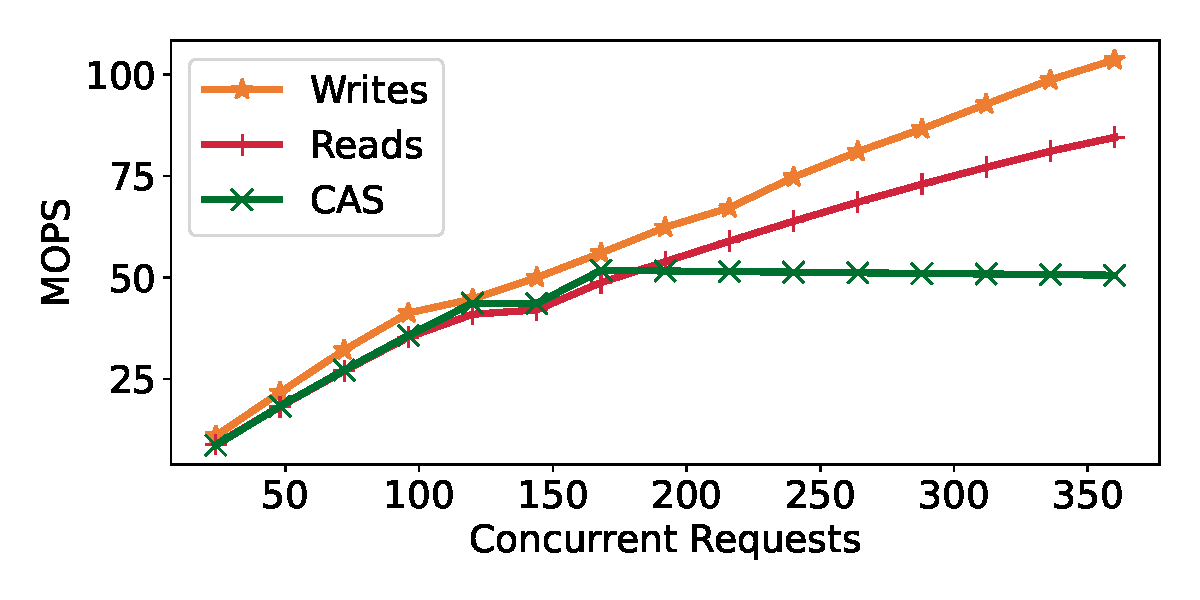
\includegraphics[width=0.485\textwidth]{fig/rdma_concur.pdf}
  \vskip -0.5em

    \caption{Achieved throughput of RDMA verbs across twenty queue
      pairs on data-independent addresses as a function of request
      concurrency.  When using atomic requests, ConnectX-5 NICs can
      support approximately 2.7 MOPS per queue pair, up to about 55
      MOPS in aggregate.}

    \label{fig:rdma_concur}
      \vskip -0.5em
\end{figure}

\begin{figure}[t]
  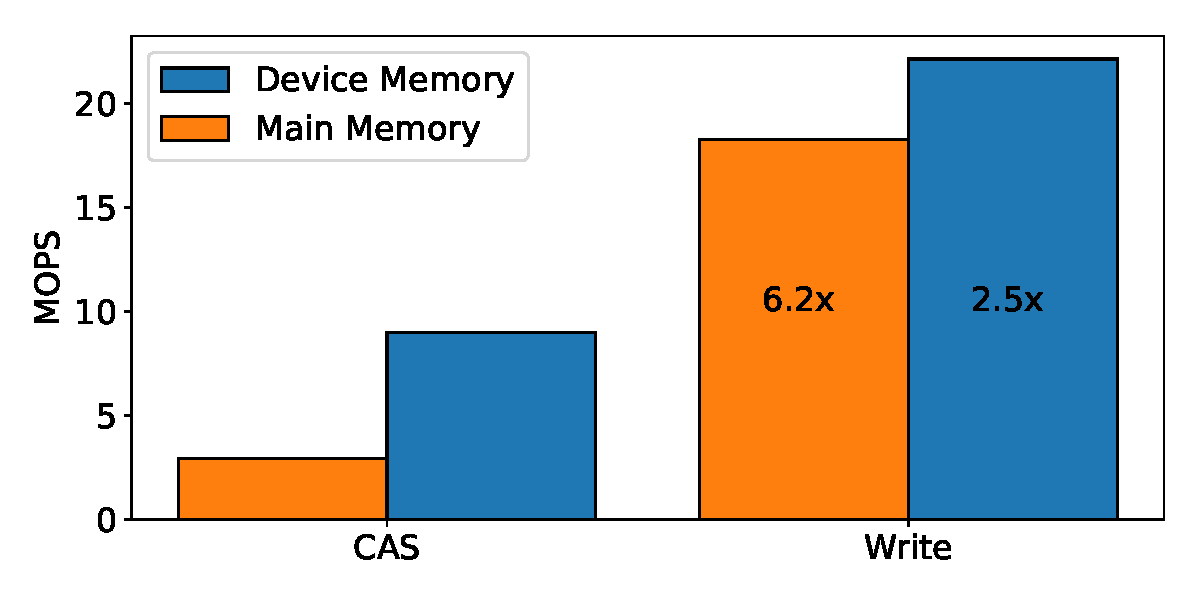
\includegraphics[width=0.485\textwidth]{fig/cas_vs_writes.pdf}
%  \vskip -0.5em

  \caption{ Throughput comparison of serialized RDMA operations in
    NIC-mapped device and main memory. Writes obtain 6.2$\times$ higher
    throughput than CAS in host memory and 2.5$\times$ higher in NIC memory despite being restricted to a single queue pair.  }

    \label{fig:cas_vs_writes}
%      \vskip -0.5em
\end{figure}

\paragraph{Remote locks}
In a remote-locking scheme, clients use an atomic RDMA operation to
attempt to aquire a lock: because the operations are totally ordered
at most one client will succeed at a time.  Unfortunately, atomics are
famously expensive~\cite{design-guidelines}, fundamentally because
they require mutual exclusion across all RDMA queue pairs---concurrent
read and write operations with a data dependency on the atomic address
must stall until the atomic completes.  Figure~\ref{fig:rdma_concur}
considers the best-case scenario where clients attempt to access
unique locks (i.e., each instruction is issued to an
isolated cache line) in remote memory using an atomic operation in
comparison to reads and writes.  We confirm that the findings of prior
studies~\cite[Fig. 14]{design-guidelines} with older hardware (i.e.,
ConnectX-3) remain true on our ConnectX-5 NICs, namely that atomic
requests scale with non-atomics only to a point.\footnote{Experiments
with a ConnectX-6 exhibit similar behavior.}  CAS operations have a
hard performance ceiling, while standard verbs (e.g., read and write)
continue to scale with increased request concurrency.  The situation
is even worse when operations target the same address (i.e., lock
contention; not shown).

%% These operations are expensive. On a single address
%% atomic instructions can only execute a few million operations per
%% second, each operation forces a blocking PCIe round trip.  As a
%% performance mitigation Mellanox NICs supply a small (few KB) region of
%% device mapped memory which allows the memory side NIC to execute RDMA
%% instructions on it's local device memory without incurring a PCIe
%% round trip~\cite{sherman}.  Executing atomics on this memory is
%% 3$\times$ higher throughput than host memory, but still slower than
%% it's read and write counterparts~\ref{fig:cas_vs_writes}.  Across
%% independent addresses they have approximately half the throughput of
%% read and write (Figure~\ref{fig:rdma_concur}).

\begin{figure}[t]
    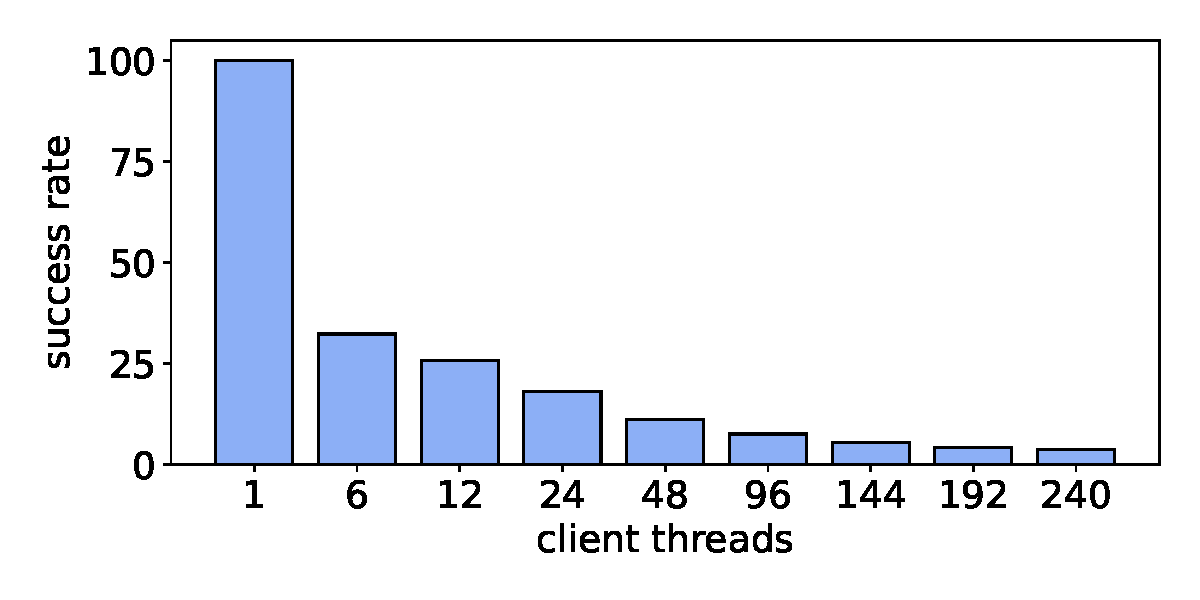
\includegraphics[width=0.485\textwidth]{fig/success_rate.pdf}
    \vskip -0.5em
    \caption{Percentage of successful operations in a
      50:50 read-write workload spread across 1,024 keys according
      to a Zipf(0.99) distribution as more client threads are
      added. At 240 threads less than 4\% of operations succeed.}
      
    \vskip -0.5em
    \label{fig:success_rate}
\end{figure}

One of the difficulties RDMA NICs face when implementing atomic operation
is ensuring that there are no other conflicting memory operations at
the server---even ones issued locally.  More generally, any
main-memory operation issued by the NIC must cross the PCIe bus and
face potential contention.  Modern Mellanox NICs like the ConnectX-5
provide a small region of on-NIC memory that can be mapped into the
address space of RDMA applications,
%.  Mapping RDMA requests onto NIC memory
removing the remote PCIe overhead for frequently accessed data.
(Indeed, Sherman employs this memory region to store its B+Tree locks.)
%but still requires atomicity across queue pairs.
Figure~\ref{fig:cas_vs_writes} compares the performance of
serialized CAS and write operations to addresses in main vs.
NIC-hosted device memory. CAS operations are issued across many
queue pairs to achieve maximum throughput while the write operations are
issued on a single queue pair to enforce serialization.
%leverage the serialization provided
%by RDMA's reliable connection abstraction to ensure in-order
%execution.
While the use of NIC-hosted memory boosts CAS throughput
from approximately 3 to around 9 MOPS, write operations remain
dramatically more efficient in either case.

\paragraph{Optimistic concurrecy.}
One way to avoid the overhead of remote lock aquisition in low-load
situations is to attempt to directly modify the data (using an
atomic RDMA operation) and recover if the operation fails due to a
race; such schemes are known as optimistic concurrency control.  While
far more performant than lock-based appraoches in the un-contended
case, optimistic appraoches can be prohibitively expensive when
contention is common.  As a concrete example we consider the chances
of success in Clover.
%Recall Clover maintains a linked list for each key and attempts to read and
%write to the tail of the list for each operation. The location of the tail of
%the list is cached at each client and used as a hint for subsequent operations.
%If the hint is stale the client obtains an updated tail pointer and retries the
%RDMA request.
Figure~\ref{fig:success_rate} shows the percentage of requests
which succeed in a 50:50 read-write workload as a function of the number of
concurrent client threads. Success rate drops dramatically as client threads
increase.

At present RDMA has no support for addressing failed operations at the
server, such as pointer chasing or retrying operations---although some
have proposed such extensions~\cite{rma,snap,prism}.  Rather, RDMA
clients are forced to resolve failures themselves at significant cost.
%In general, the conflicting operation(s)
%must be retried incurring additional latency and bandwidth.
In some
systems, the retry is a heavyweight, pessimistic operation, leading to
a substantial---but fixed---overhead.  In others, like Clover,
subsequent attempts remain optimistic, resulting in a linear
(per-retry) increase in costs.  In the latter case, very high
rates of contention can lead to congestion collapse, where a retry is
essentially doomed to failure, dramatically decreasing system
throughput.
%

%\paragraph{Bandwidth inflation.} 

Concretely,
%One of the most direct impacts of failed requests is the bandwidth
%overhead of the retries.  Because a Clover operation actually
%consists of multiple RDMA requests, the total bandwidth is not
%strictly proportional to the failure rate, but rather slightly
%sub-linear.  Nevertheless, the expected cost of each operation rises
%steadily with contention, which is a function of both the workload and
%level of concurrency.  Our
our measurements show that under contention the
average bandwidth cost of Clover read and write operations can inflate
by 16$\times$ (Figure~\ref{fig:bandwidth_reduction}) when compared
to an optimal scenario in which all operations succeed on their first
try.
%
%\paragraph{Tail latency.}
%
Perhaps even more significant than the overheads associated with the expected
number of retries is the cost at the tail---namely the latency associated with
those particularly ``unlucky'' requests that fail repeatedly.  Note that these
operations are precisely those for hot memory locations, so likely to be
ones that matter.  Under contention
%(e.g., 50\% write operations with 396 threads)
Clover's 99th-percentile tail latency increases by
over 300$\times$ (Figure~\ref{fig:tail_latency}) in our experiments.



\subsection{Implications}

Systems that leverage RDMA atomics have hard performance
limits because the aforementioned constraints.  Locks
located at a single address which use traditional lock,
unlock operations are limited to around 500k accesses per
second. This assumes perfectly coordinated requests, under
contention requests which fail to acquire or release a lock
still consume operation bandwidth.
%%
Under contention RDMA has poor support for traditional
locking. In contrast optimistic data structures with locks
scattered throughout, such as a linked list, are not rate
limited by this single address restriction.  However, they
are fundamentally limited by the fact that any atomics have
half the throughput of reads and writes. More critically,
under contention optimistic data structures have no liveness
guarantees.

%% We measure the failure rate of optimistic reads
%% and writes to a shared linked list. Operations are reads and
%% writes to the tail of the list, all writes are appends.
%% under contention atomic operations fail frequently
%% (Figure~\ref{fig:success_rate}).

%%



\section{\sword}

\sword\ is our general-purpose approach to accelerating RDMA-based
applications like shared disaggregated memory that require operation
ordering across clients.  In this section we explain the functionality
\sword\ provides and then apply it to two separate remote memory
systems.  At a high level, \sword\ is capabile of 1) tracking on-going
reliable connections, 2) parsing and caching their contents, and 3)
modifying operations in flight.  Because it defines a total order on
outgoing RDMA requests, \sword\ can safely remap them between
different connections as well as transform atomics into lightweight
verbs.  As we show in the context of Clover, by tracking a small bit
of application-specific state, \sword\ can also use its knowledge of
operation order to modify the target address or value of conflicting
operations to resolve write/write conflicts before they occur.

%%
%% These techniques are implemented in a DPDK prototype for the
%% lock based approach and fully realized in P4 for optimistic
%% data structures. Figure~\ref{fig:system} shows the overall
%% design of {\sword}.

% Locks are
% managed in network, and the results of locking operations
% are forward to memory. Lock accesses are accelerated by
% replacing RDMA atomic operations with writes in flight.
% Modified lock operations are multiplexed onto existing RDMA
% connections, per lock, to ensure serialized access to the
% lock. {\sword} also provides a mechanism to remove
% contention from optimistic data structures by caching the
% metadata required to detect and resolve conflicts. 

% In all cases switch memory and compute are highly
% constrained. Any operations that exceed the processing
% limit of the match action pipeline require recirculation
% which consumes additional switch bandwidth. 

%\subsection{RDMA processing}

\begin{figure}[t]
  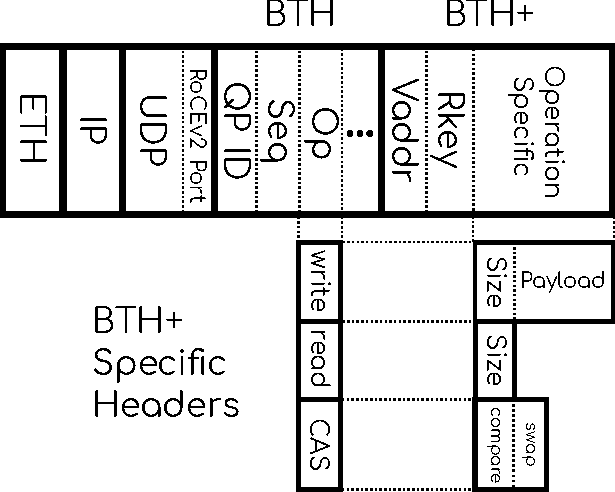
\includegraphics[width=0.485\textwidth]{fig/rocev2.pdf}
  \vskip -0.5em

    \caption{ RoCEv2 headers consist of an Ethernet, IP, and
    UDP header, a special UDP port denotes that the packet
    is RDMA. The RoCE BTH header stores QP data, sequence
    numbers, flags, and operations. The BTH+ header follows
    and stores operation specific data such as virtual
    addresses, DMA size, and compare-and-swap payloads.
    }

    \label{fig:roce_header}
      \vskip -0.5em
\end{figure}

\subsection{Connection multiplexing}

RoCEv2 tunnels the original Infiniband-based RDMA protocol on top of
UDP, using destination port 4791.  RoCEv2 packets have two headers,
BTH,and BTH+, shown in Figure~\ref{fig:roce_header}, both of which
\sword\ needs to parse.  The BTH header indicates the operation, while
the BTH+ headers contains the target virtual address and the operation
payload.
%
%% \sword\ uses reliable connections to ensure that packets are
%% not reordered after atomic operations have been resolved. By
%% default, RoCEv2 packets on separate QP can be reordered on
%% the NIC, or on PCIe, therefore swapping CAS operations to
%% Write on the switch leads to an unsafe race condition
%% (Figure~\ref{fig:reorder}).
%
In cases where \sword\ wishes to enforce ordering across operations
from different clients, it multiplexes them onto the same reliable
connection.  \sword\ does not establish or terminate connections
itself---setup and teardown are handled end-to-end as usual by the
RDMA NICs.  Rather, \sword\ simply moves operations between existing
connections.

\begin{figure}[t]
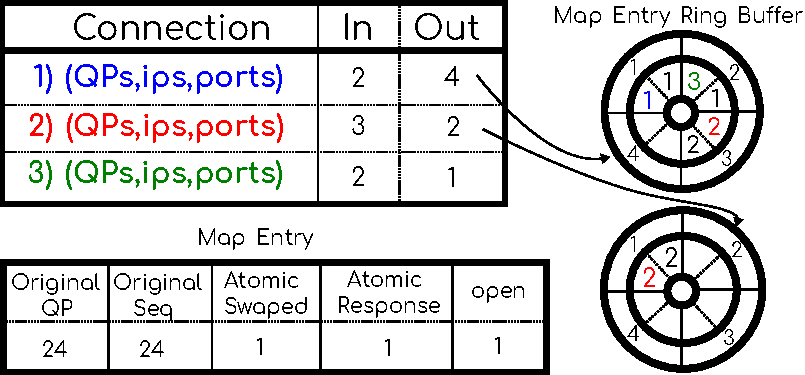
\includegraphics[width=0.485\textwidth]{fig/connection_multiplexing.pdf}
\vskip -0.5em

    \caption{ Queue pair mapping data structure. Each RC
    connection has metadata stored statically per
    connection. Sequence numbers are dynamic per connection,
    \sword stores both incomming and outgoing sequence
    numbers for each connection. Stubs for each outgoing
    request are stored in a fixed sized circular buffer.  }

    \label{fig:qp_mapping}
      \vskip -0.5em
\end{figure}

\paragraph{Connection tracking}
%
To facilitate connection multiplexing, \sword\ maintains a table of
reliable connections transiting the switch, shown in
Figure~\ref{fig:qp_mapping}.  Connections are uniquely identified by
their source and destination IP address, source UDP port (the
destination port is fixed for all RoCEv2 traffic), and queue pair ID.
Entries are added to the table upon queue pair establishement and
removed at teardown (or after a timeout).  Each row in the table is
associated with a ring buffer of \emph{map entries} that track
outstanding operations.  As RDMA packets arrive and are placed into a
total order at the switch, the row corresponding to the packet's
incoming queue pair is updated with the current sequence number.
Retransmissions (i.e., packets whose sequence numbers are no greater
than the value already in the table) do not cause the table to update.
The table also records the highest sequence number used by an outgoing
packet on each connection; this need not be the same as the incoming
sequence number due to remapping.

\paragraph{Remapping}
\label{ss:remapping}
In general, RDMA packets will be forwared using the same connection on
which they arrived.  In application-specific cases, however,
\sword\ may wish to move them to a different queue pair, i.e., to
multiplex them onto a shared connection.  In that case, the packet
needs to be rewritten to use the new connection's source and
destination addresses (both IP and Ethernet), UDP port, and an
appropriate sequence number---which is computed to be one higher than
the last packet transmitted on the outgoing connection.  (Incoming
retransmissions---detected due to their non-advancing sequence
number---are always mapped to the same outgoing connection and
sequence number as the original.)  To facilitate ACK and
retransmission handling, every packet creates a map entry in
the ring buffer associated with its outgoing connection.

For efficiency, we maintain the ring buffers as fixed-size arrays and
use the packet's outgoing sequence number (modulo the buffer size) as
an index.  Each entry contains a reference to the packet's incoming
queue pair, its original sequence number, and, in the case of atomics,
space to record whether the operation was replaced by
a write (Section~\ref{ss:rewrite}) and, if so, the prior value of the
target address---which is tracked using application-specific logic
discussed below.
%
%% Map entries are sufficient for bookkeeping packets, but many
%% packet fields must be updated to ensure that the RDMA NICs
%% accept the packets as valid.
%% To multiplex a
%% packet to another connection we update the packet's IP
%% addresses, udp sender port, queue pair, and sequence number
%% then forward the packet as normal. Without applying these
%% updates the receiving side NIC will either reject the
%% packet, trigger go-back-n, or generate an error. 
%% %
%% On mapping the
If the packet was remapped, both the invariant CRC (ICRC) of the RDMA
packet and the IP checksum must be updated.  
%%


\paragraph{ACK coalescing}
De-multiplexing ACKs for remapped operations is non-trivial due to
optimizations in the RDMA protocol. Specifically, an RDMA NIC may
coalesce ACKs to reduce the number of packets transmitted and save
bandwidth: like TCP, ACKs are cumulative. Coalescing presents a
challenge when operations from multiple incoming connections are
multiplexed onto another, as an ACK may correspond to operations
issued by more than one client.  Forwarding the ACK back to only the
client who issued the (last) operation referenced in the ACK will
cause the other clients whose operations were implicitly acknowledged
by the server to timeout and retransmit.  Conversely, forwarding ACKs
to clients without outstanding operations could lead to unspecified
behavior.
%
%is a problem when multiplexing to two or more
%clients. A request from one client, may cause the coalescing of a
%result for another. If this occurs the second client will not receive
%a response and eventually time out, leading to retransmission and high
%tail latencies.
%%
Upon receipt of an ACK, \sword\ consults the map entries in the ring
buffer for the relevant connection.  \sword\ generates a separate ACK
for each incoming connection with outstanding packets acknowledged by
this ACK, setting the sequence number (and address and queue pair
information) according to their map entries.

%% \sword\ detects ACK coalescing by monitoring response packets. If a
%% higher number ack is received we know by the guarantees of RC that the
%% lower packets operation was executed and it is safe to generate an
%% ACK. Mapped requests for the missing packet are used to generate the
%% ACK.
%% %
%% Multiple acks can be coalesced so
%% this processes is recursive when ack coalescing is detected.
%% This processes is not required if response coalescing is
%% turned off.

\subsection{State caching}

In addition to connection information, \sword\ can also parse RDMA
operations to track the current state of memory locations of interest.
The particular addresses are obviously application specific, but the
mechanism is generic: \sword\ simply needs to apply the operations to
its local cache in the same order it transmits the operations to the
destination.  We find that despite the large amounts of data
transferred by passive memory systems, contention is typically
localized to a few key addresses, such as those that are used to store
locks, indexing datastructures, and other metadata.  Moreover, these
locations are typically accessed using atomic operations, limiting
the data size to eight bytes a piece.

%% maintains a cache of application data to resolve
%% conflicting operations. The contents are application
%% specific, in our evaluation we use a cache of locks, and
%% key-value locations. The cache consists of named p4
%% registers -- named variables mapped to pipeline stages which
%% persist across packets. The size of the cache depends on the
%% application, switch space is limited, so only contended
%% resources are cached. In our evaluation contended resources
%% are known a priori, however that could be dynamically
%% selected a runtime using LRU or heavy hitter detection.

% Application caches are distinct
% from the contention resolution technique. We use cache to
% store both locks, and key value information for both Clover
% and Sherman.



\subsection{Atomic replacement}
\label{ss:rewrite}

When \sword\ tracks the state of address locations of interest, it
necessarily determines outcome of atomic operations.  Hence,
\sword\ can be configured to multiplex all operations targetting
specific addresses to the same connection and replace atomic
operations with writes that simply store the outcome of the atomic,
whether it be a compare-and-swap or fetch-and-add.  Here we describe
how \sword\ handles the former without loss of generality.

Replacing a CAS operation with a write is straightforward as the
RoCEv2 headers differ by only a few fields
(Figure~\ref{fig:roce_header}).  \sword\ transforms CAS requests to
writes by swapping the BTH OP code, setting the BTH+ size field of the
write to eight (recall all CAS operations are 64-bits long), and
copying the appropriate value---either the ``swap'' value from the CAS
operation on success or the current (cached) value on failure---into
the payload.  \sword\ indicates the operation has been transformed in
its map entry (Section~\ref{ss:remapping}) as well as recording the prior value.
Because a write's size field is only four-bytes long (as compared to
the second 64-bit compare field in a CAS operation), the length of the
packet shrinks by four bytes; \sword\ updates the IP length field
accordingly.

%% details the difference between WRITE and CAS headers. When
%% mapping the virtual address and remote key remain the same.
%% We modify the opcode in the BTH header from WRITE to CAS
%% which instructs the memory side nic to treat the packet as a
%% write.  CAS is predefined to be 64 bit, so we install a
%% write header with a DMA length of 8, and a payload with the
%% tie breaker value. Note that the value set is application
%% specific. In the case of locking, the result is the locks
%% value after the operation is attempted. Finally the packet
%% length is truncated as write packets are 4 bytes shorter
%% than CAS packets.

%% From a RoCEv2 perspective
%% the per-packet transformation from CAS to write can be applied easily
%% in the data path; RoCEv2 CAS and write headers only differ by a few
%% fields. CAS can be thought of as a special case of a write, where the
%% write is conditional and the length is preset to 8 bytes.
%% %%
%% %so the modified packet will not be
%% %rejected by the memory side NIC.
%% The transformation from CAS to write
%% is deterministic and only requires a few cycles to transform the
%% header.

After processing the write operation the destination NIC will respond
with a regular, write ACK. As part of its ACK processing, {\sword}
applies an inverse transformation to convert write ACKs to Atomic ACKs
when necessary.  RDMA Atomic ACK headers are very similar to regular
ACKs with the only difference being that the atomic ACK contains the
value that was overwritten, which \sword\ retrieves from the
corresponding map entry.


\subsection{Disaggregated memory}

We now describe how we use \sword's techniques to accelerate the
contention management techniques used by Sherman and Clover.
%We present {\sword} an in-network solution for sharing
%remote memory. {\sword} enables sharing by providing two
%forms of application specific serialization. The first of
In the case of Sherman, \sword\ multiplexes all operations (encoded as
CAS operations) for a given lock on a single connection, caches lock
state at the switch, and replaces aquisition attempts with writes.
%
%% 's ability to 
%% which is to resolve atomic operations in network. Using a
%% cache and application logic \sword\ determines the result of
%% the atomic operation, and forwards the result to memory as a
%% write. RDMA RC connections are used to ensure that resolved
%% operations are not reordered downstream.
%
\sword's acceleration of Clover is more lightweight---in fact,
entirely soft-state---but even more impactful.  By caching a small
amount of server state that clients manage through CAS operations,
\sword\ is able to adjust these requests to ensure they succeed at the
server, thereby avoiding expensive application-level retries for
concurrent updates.
% \sword caches updates to the shared structures and
% modifies stale requests in flight with the most up to date
% information removing the need for operations to fail. 
%% These mechanisms are used to accelerate locks in
%% Sherman~\cite{sherman} and remove all contention from a
%% key-value store, Clover~\cite{clover}.

\subsubsection{Shared locks}
\label{sec:locking-algorithm}

Sherman uses CAS operations to implement its node locks.
%Sherman and future far memory systems like Sherman which use lock based
%approaches to guard remote data will incur the cost of using RDMA atomics. 
%
%Implementing locks with CAS is straightforward, the following algorithm is
%common and is used to implement locks for nodes in Sherman. The
%CAS operations are of the form \texttt{CAS(old\_value,new\_value)}.
Sherman's locks are simply specific (NIC-hosted) memory locations that
store either a one (locked) or zero (free).  Hence, lock requests are
expressed as \texttt{CAS(0,1)}, which fail if the lock is unavailable
(i.e., the stored value is currently not 0) or atomically set the
value to 1---acquiring the lock---if successful. Unlock operations are
the inverse.  Presuming communication between the ToR and the memory
server is reliable and in-order (as provided by an RDMA reliable
connection), it is conceptually straightforward for \sword\ to cache
the current value of the lock at the ToR.

In our design, \sword\ muliplexes all operations for a given address
(i.e., lock) over the same connection to maintain ordering between the
ToR and destination server.  It can then use its local cache to
determine whether an arriving CAS operation will succeed or fail.  (If
it does not have the current value at the target address cached, it
allows the atomic to pass through unmodified and populates its cache
with the response.)  Knowing the outcome, \sword\ is free to replace
the CAS operation with a lightweight write in flight.  When a CAS
operation arrives for a lock address, \sword\ replaces it with a write
for the specified value.  (Releases will always succeed, setting the
value to 0, while lock acquisition attempts always leave the value as
1; their succes or failure is dictated by the prior state.)  When the
ACK comes back, \sword\ converts the ACK to an Atomic ACK before
forwarding it back over the original connection to the client.
Because lock values are always zero or one, it sufficies to store a
single bit---as opposed to eight bytes---to record the prior value in
a lock operation's \sword\ map entry.

Even in the case when the lock is already held (and the aquire attempt
is doomed to fail), \sword\ still forwards a write request to the
memory server to ensure the client and server agree regarding the
total number of RDMA verbs communicated between them.  The ACK
is replaced with a CAS ``failure'' so that the sender knows the lock
acquisition failed.  This is in keeping with \sword's
performance-enhancing-proxy philosophy: it accelerates, but does not
replace, the application's end-to-end semantics.
%Again, unlock is similar.
Indeed, one could implement the lock server at the ToR
itself~\cite{netlock}, but that would require a redesign of the
underlying system; our goal is to support selective deployment where
\sword\ may not be on-path for all servers, dictating that we do not
make any changes to the existing system.  Moreover, our approach does
not require terminating RDMA connections at the switch, which would
require extensive buffering.


% One might ask why not host all locks on the switch thereby
% reducing bandwidth to end hosts and saving latency? By forwarding all traffic to
% the memory servers, memory can still act as ground truth for the state of shared
% data. If a switch were to be reset, no lock state is lost. Further it allows for
% optimizations, clients can read shared structures and determine what data is
% locked by inspecting memory with reads directly. This saves implementing
% potentially complex read and write logic for all data structure access on the
% switch, and prevents it from becoming a single point of failure.


% The combination of read and write steering dramatically improves the
% performance of Clover (as shown in Section~\ref{s:results}), but only
% scratches the surface of the potential improvements for far memory
% systems.  


%Atomic replacement only works when all operations---across all client
%connections---that share server state are vectored to the same queue pair.
In
general, the determination of which operations share state is application
specific and requires inspecting each packet to extract the relevant pieces
of metadata. In the case of Sherman, lock locations can be identified by
inspecting CAS requests. Each CAS virtual address corresponds to a node lock in
the Sherman B+Tree.
%%While removing locking operations is a general principle here we consider a
%%solution for RDMA.  %Different transports with different ordering guarantees
%%would require bespoke solutions.  
%The challenge, of course, is that the RDMA specification stipulates that each
%client establish its own queue pair with a given server, so operations for a
%given lock from different clients will arrive at the ToR on distinct queue
%pairs.
While \sword\ must interpose on the full set of queue pairs terminated
by a given (set of) server(s),
%and vector operations to queue pairs accordingly.
this seems reasonable as the ToR is usually on-path for all servers in disaggregated rack settings.

\sword\ is designed for closed looped clients. Connection
remapping could require large amounts of buffering in
network if clients had many in flight requests spread across
multiple QP. Out-of-order requests would need to be buffered
prior to delivering them. Out-of-order packet delivery
triggers RoCE's go-back-$n$ retransmission protocol.
%% Storing connection information could lead to a potential
%memory bottle neck. 
Our aim is to enable rack-scale disaggregation where the
total number of cores (clients) is less thant O(1k). Here
the few MB of available switch memory is more than
sufficient for storing connection metadata.

%to support go-back-$n$ retransmissions.

%
%This technique does not reduce contention on the lock, but simply removes the
%CAS hardware bottleneck. An alternative approach to this locking scheme would b%e
%% to use the switch as a lock server similar to
%% Netlock~\cite{netlock}.~\todo{help!}Our goals are orthogonal to
%% Netlock as we want to accelerate existing protocols, not require any
%% end host code modifications, keep switch logic to a minimum, and
%% maintain only soft state on the switch. By propagating requests to
%% end hosts we ensure that no state is lost on switch failure. And
%% that any async read operations can be issued to remote memory
%% directly without needed to be interpreted by the switch.  By
%% Forwarding all requests we remove the need for the switch to
%% implement go-back-n retransmissions. The switch is only required to
%% store the current state of the lock, and track outstanding requests
%% to modify their return values. In the following section we will see
%% that tracking outstanding requests is required when swapping CAS to
%% write across multiple connections.

\subsubsection{Steering}
Unlike Sherman, Clover does not implement locks.  Instead, Clover
attempts to append to a per-key linked list using atomic operations.
Clover detects concurrent updates by breaking writes (i.e., list
appends) into two RDMA operations: one write to create a new node, and
a CAS operation to update the next pointer of the node at the tail of
the list---the latter fails when another node was added concurrently.
Concretely, it uses CAS operations to attempt to replace a
\texttt{NULL} pointer (indicating the end of the list) with a pointer
to a new element.  To prevent such stale CAS requests from failing,
{\sword} maintains a cache of the location of the (next pointer of
the) node at the tail of each key's linked list. If a CAS request
arrives at {\sword} destined for a stale virtual address (i.e., an
address other than the one currently cached for that key), {\sword}
\emph{steers} the CAS operation by replacing its target address in the
BTH+ header with the cached address.
%% CAS operations that ``lose'' a race will find a
%% non-\texttt{NULL} value at their target address and force the client
%% to retry at the new end of the list.  \sword\ can avoid these failures
%% by \emph{steering} the target address of CAS operations to what it
%% believes to be the current tail of the list.  
While \sword\ could multiplex these operations on a shared connection
to enforce ordering (and replace them with writes), our evaluation
shows the probability of reordering with a contending operation on a
separate connection after departing the ToR is sufficiently low that
the remaining cost of (clients) resolving such failures is minimal.

%% Recall that writes in Clover are destined to the presumed tail of a
%% key's linked list, but the target of any individual RDMA request may
%% be out of date due to races with concurrent updates.



%% Here, \sword\ need not incur the overhead
%% of connection multiplexing;   

%% Recall Clover takes an optimistic approach to concurrency control
%% Unlike connection multiplexing, steering does not modify the
%% RDMA operation. Steering is used when atomics are not
%% applied to a single address. The atomic bottleneck on
%% independent addresses is only half of that of reads and
%% writes, in most algorithms less than half of operations are
%% atomics, therefore the bottleneck is never reached. 
%%
We implement steering by maintaining a cache of (a subset of) Clover's
linked-list datastructures.  %% , and data structure specific code for
%% resolving conflicts. 
When a Clover packet arrives at the switch, it is parsed and passed to
application-specific cache management code that extracts the
salient information from the payload.
%While conceptually simple, the actual implementation is somewhat
%involved due to the design of both Clover and the RDMA protocol and
%our desire to remain transparent to both.  Specifically,
Unfortunately, Clover RDMA CAS requests do not explicitly specify the
write operation to which they correspond; {\sword} infers the
operation by checking the size of the RDMA request and then extracts
the Clover key from the appropriate the location in the packet.  The
key is used as an index into a lookup table to find the virtual
address of the current tail node for that key.  Our strategy requires
64 bytes of data per key---the size of an RDMA virtual address.


%% While the semantics are
%% application-specific in our evaluation we find it simple to do without
%% making modifications to Clover itself.

%% Concretely, the target adddress of Clover writes (encoded in CAS
%% operations) is looked up in the cache. If the packet requires steering
%% (i.e., the cache indicates that the targetted address no longer
%% contains \texttt{NULL}) the virtual address in the BTH+ header is
%% updated to the cached address.  The cache is similarly updated to
%% reflect the addition of the new node.




%% %%
%% Reads and write are handled differently. Write contain
%% application specific data in the payload. This information,
%% along with the virtual address is usually sufficient to
%% identify the packet type specific to the application and
%% apply steering. 
%%

While write steering sufficies to avoid write/write conflicts,
concurrent reads face a similar dilemma: Clover reads seek to access
the current tail of the linked list, but the address may be stale if
they ``lose'' a race with a concurrent write.  To improve performance,
\sword\ similarly steers reads to the correct tail address.

Unfortunately, unlike writes (which are easy to identify by their use
of the CAS operation), Clover reads are simply RDMA read operations
for a virtual address and a length.
%While Clover 
%writes contain the key
%to which they pertain---which allows for a table lookup---
%Unfortunately Clover's
%RDMA read requests only contain the target virtual address and a size.
%When a
%read fails it must be retried, as mentioned earlier reads are
%performed iteratively until the tail of the list is reached, which in
%the case of highly contested keys could be arbitrarily long. Repeating
%reads does not destroy system performance as they are lockless,
%however in terms of client latency each retry adds serious
%latency. What makes handling reads hard is identifying the clover key
%for which the read is for, without additional data in the packet the
%value must be determined another way.
As reads can be for arbitrarily old virtual addresses a naive solution
that stored the lineage of each key would effectively require caching
the entire contents of Clover's metadata server.  Instead,
\sword\ hashes the address of each write into an array somewhat larger
than the size of the key space and stores the key along with the
address.  Collisions are resolved by replacing the old
%address
%and key with the new values
entry, allowing keys with higher update rates to
maintain longer histories in the table.

When reads arrive {\sword} looks up their destination address in the
table; if the address has a hit the associated key is used to look up
the current tail in the write cache and the RDMA read is steered to
the cached location.  Should a miss occur---either because the hash
bucket was overwritten by another key, or because the tail address is
not cached---the read is left unmodified.  If it fails to arrive at
the current tail, Clover's end-to-end recovery mechanism kicks in
looks up the last known address at the metadata server, then repeats
the processes.

%% If reads are destined to a stale location, we steer them to
%% the correct location simply by modifying the virtual address.
%% %%
%% Our implementation of \sword requires no modification to the
%% existing systems, however we note that future systems
%% codesigend with \sword in mind could reduce the in network
%% memory footprint by fingerprinting their packets with id's
%% for {\sword}.

\subsection{Failure handling}

\sword\ collocates functionality---and therefore shares fate---with the
top-of-rack switch: if \sword\ fails, connectivity was already
disrupted (i.e., the ToR is down).  Hence, the fact that a
\sword\ failure will reset all remapped RDMA queue pairs to the
attached servers seems of little additional consequence.  In the case
of steering, however, we note that \sword\ does not maintain any hard
state: failure simply results in a performance hiccup if packet-level
connectivity can be maintained.  The upshot is that a complete
\sword\ failure does not introduce safety concerns in any event.

However, there are other failure scenarios to consider.  In
particular, we presume that the ToR sees the exact stream of packets
that will be received---and processed---by attached servers.
Unfortunately, this may not be true due to packet loss (e.g., due to
CRC failures or queue overflow) or even bugs on the server.  Of
course, these failure cases exist even without \sword, and Sherman and
Clover both provide their own error handling.  The key distinction,
however, is that \sword\ maintains a cache that may become
inconsistent with an attached server, which was previously the single
authority of both application and RDMA connection state.


At an application level, Clover never acquires any locks so failures
do not result in resource stranding, and Sherman periodically detects
if locks were kept by a dead client.  At the connection level they
both rely upon RDMA to provide reliable, in-order delivery of their
messages on a per-client basis and react to failed CAS operations by
retrying their operations.  {\sword} must therefore be able to detect
and properly handle packet retransmissions; in particular \sword\ must
not treat a retransmitted packet as a new operation.  Hence,
\sword\ tracks the most recent sequence number on each QP, the
transformation it applied (remapping or steering), and whether the
operation was ACK'd by the server.  Upon retransmission
\sword\ re-applies the previous transformation.

%QP ordering ensures retransmissions are , and RDMA
%go-back-$n$ is triggered if any message is lost.

\textbf{Enforcing ordering.}
Managing responses when mapping queue pairs is somewhat more complex.  If a
packet is dropped between \sword\ and a server and \sword\ maps a subsequent
request from a different client onto the same QP, the server will generate a
go-back-$n$ response and any other in-flight requests on that QP will become
invalidated.  Hence, when {\sword} sees a go-back-$n$ ACK, it triggers the same
mechanism used for ACK coalescing but in reverse: it broadcasts a go-back-$n$
ACK to all clients with outstanding messages.  While this approach amplifies the
performance impact of a lost packet, we expect such scenarios to be unlikely in
practice.  Indeed, no packet drops ever occurred between {\sword} and a server
during our experiments because our clients issue only closed-loop operations.

\textbf{Conflict avoidance.} Without queue-pair mapping, there are
fewer concerns at the connection level, but \sword\ must now be aware
of potential inconsistency between its cache and server state.
Concretely, in the case of Clover, it is possible for a linked list to
become ``broken''.  If \sword\ sees a client issue a \texttt{CAS(A,B)}
request (attempting to append node $B$ to the list at $A$) before
another issues \texttt{CAS(A,C)} (appending node $C$ to the
same---stale---tail), \sword\ will steer \texttt{CAS(A,C)} to
\texttt{CAS(B,C)}. If the \texttt{CAS(A,B)} operation is lost between
\sword\ and the server, \texttt{CAS(B,C)} will still succeed, causing
a broken chain: the pointer $A\rightarrow B$ does not exist but
$B\rightarrow C$ does, and {\sword} believes $C$ to be the tail.

In the normal case, the client will timeout and retransmit
\texttt{CAS(A,B)}, which \sword\ will identify as a retransmission and
\emph{not} steer to the ``new'' tail, thereby repairing the list.  (In
the mean time, the missing link is immaterial because
subsequent requests are being steered by \sword.)  If, however, the client
were to fail prior to retransmitting the CAS the chain will remain broken.
Here we use an out-of-band mechanism to repair the chain: on occasion
our control plane queries the switch to check for outstanding CAS
requests and simply retransmits them (spurious retransmissions are
handled gracefully by the server).  The trickiest case is if
\sword\ itself also fails in the mean time: we defer protecting
against this double-failure scenario to future work.





% {\sword} caches locks and forwards the result of locking
% operations to remote memory. Storing locks in switch memory
% enables 10's of millions of lock and unlock operations per
% second~\cite{netlock}. At these rates CAS on single
% addresses is the bottleneck. {\sword} serializes lock
% access and forwards the results to the servers, therefore
% the application CAS operation can be modified to a simple
% write as the result is known prior to arriving at the memory
% side NIC. On an individual QP this modification is safe --
% across QP however reordering can occur between the switch
% and memory. We therefore multiplex lock operations onto
% shared QPs.
% %%
% Swordbox manages reliable connections for all connected
% clients. When clients first connect {\sword} detect the
% connection startup and tracks the sequence numbers on that
% connection. The total number of active connections is
% tracked as well. When a lock acquire or release issued {\sword}
% take the lock address \textit{mod} it's address and assigns
% it to a connection. This ensures that all operations to the
% same lock are placed on the same reliable connection.
% %%
% When a CAS for a known lock passes through {\sword} it checks
% it's lock table and calculates the result of the locking
% operation, (aquired, released or failed). The RDMA packet
% then has it's operation value changed from CAS to Write, and
% is assigned to the downstream reliable connection the lock
% was mapped to. Each request must be multiplexed and
% demultiplexed, when a lock request is assigned to a stream
% it has it's QP, and sequence number updated so that the
% receving side NIC is unaware that any modification have been
% made in network. A stub of the mapping is stored with
% relation to the connection, when a response from the NIC
% returns from the switch the packet has it's sequence number
% mapped back to it's original value, and is mapped back to
% it's original sender. For each mapped request the switch
% must store both a sequence number and the id of the
% requesting client. 
% %%
% Our systems support only closed loop clients which issue one
% request at a time, and are guaranteed to retry requests lost
% in transit. Using this assumption the amount of state the
% switch needs to store is bounded by the number of clients.
% It must store a sequence number for each client QP, and
% stubs for each outstanding request. This requires at most 2
% 24 bit sequence number for each client.


% \subsection{Optimistic Concurrency}

% \subsection{Steering}

% Lock based data structures are limited under contention both
% by the rate at which locks can be acquired, and by the size
% of the critical section each client must execute. Under
% severe contention the critical section is the bottleneck.
% Optimistic strategies differ in that work completed in
% scratch memory, and then committed via an atomic operation
% like CAS. 

% Take for example a linked list which supports an append
% operation. Clients running append must first write the
% value of the node they wish to append, and then commit to
% the list by running a CAS which modifies the null pointer at
% the end of the list to then point to the new entry. Such
% strategies require no lock acquisition but still struggle
% under contetion. If the end of the list is continuously
% being appended to and multiple clients are in a race, one
% will succeed, the others will fail, need to traverse the
% list to the new tail, and reissue a request. 

% {\sword} is designed to entirely remove contention in
% optimistic concurrency schemes. As all requests are
% serialzed {\sword} can observer the most up to date location
% of the lists tail. We cache this value and use it to resolve
% conflicts. When requests arrive at sword which append to the
% tail of the list, the virtual address of the tail is stored
% for that key. This requires storing one 64 bit virtual
% address for each key in the key value store. While this
% overhead may seem large, {\sword} need only store hot keys.
% Uncontended keys can simply be written and read using
% clovers default protocol. When requests for a key arrive at
% {\sword} it looks up the value of the write and determines the
% location of the lists tail. If the request is pointing to
% the tail, the in network cache is updated and the request is
% forwared to memory with no modification. If the request is
% out of date (directed to an interior node of the list)
% {\sword} modifies the virtual address of the CAS and forwards
% it to the known tail location, updating it's own cache in
% the process.


%% \subsection{Example Systems}

%% We implement both of our contention reduction strategies in
%% two disaggregated systems Clover, and Sherman. 
%% %%
%% \textbf{Sherman}: is a B+ tree built for one sided RDMA.
%% Shermans core mechanism for mitigating write conflicts is a
%% lock table mapped to the memory side NIC. We emulate
%% Shermans lock table and demonstrate \sword's ability to
%% improve performance by placing the lock table in network and
%% mapping CAS operations to writes using our connection
%% remapping technique. We use our DPDK implementation of
%% \sword in our evaluation of Sherman.
%% %%
%% \textbf{Clover:}: is a key value store built for one sided
%% RDMA. One sided operations read and write updates to the
%% store by appending to keys structured as linked lists. Under
%% contention both reads and writes fail as the tail of the
%% lists move. We use \sword's ability to cache the most up to
%% date tail and steer requests to the correct location to
%% remove all contention from both reads and writes enabling
%% the performance of raw uncontended RDMA operations. Our
%% evaluation of Clover is performed using our P4
%% implementation of \sword.


% \textbf{sherman:} {{\sword}} assumes that locks are located at well known
% location. Logic for managing locks is application specific
% and implemented in {\sword}. No modification to the client is
% required as {\sword} operates directly on RDMA packets, using
% their QP id's and virtual addresses. In Sherman for instance
% locks are mapped to a special region of NIC memory with a
% well known virtual address range.

% \textbf{Clover:} This is the exact scheme Clover uses to
% handle writes to its persistent key value store. Clover
% operates well under read only workloads but struggles under
% contention as the tail of each list moves faster clients
% must repeatadly chase the tail pointer of the list, each
% read requiring a round trip.

% This strategy remotes all contention from Clover and
% requires not modifications to the application itself. A key
% aspect of this approach is that Clover has end to end
% recovery and does not rely on {\sword} to complete requests.
% If a key is not tracked by {\sword} then the request is
% forwarded directly to memory with no modifications. 

% Our
% prototype statically tracks hot keys, however a dynamic
% solution in which hot keys are detected via a count min
% sketch are well within the capabilities of future
% versions~\cite{switchml}.
